\section{Auswertung}
\label{Auswertung}
In Diesen Kapitel sollen die Aufgenommenen Daten ausgewertet werden
\subsection{Bestimmung von Materialeigenschaften}
Für den Versuch stehen vier Metallstäbe, zwei runde und zwei Eckige, zur verfügung. diese
wurden jeweils gewogen und ausgemessen die Ergebnisse sind in \autoref{tab:eigenschaften} zu sehen.
Die Dichte $\rho$ berechnet sich, mit Länge $L$ und Durchmesser $d$, für die runden Stäbe über:
\begin{center}
    $\rho=\frac{4m}{d^2L}$
\end{center}
und für die eckigen Stäbe, mit Seitenlängen $a$ und $b$ über:
\begin{center}
    $\rho=\frac{m}{abL}$
\end{center}
der Messfehler berechnet sich dann über die Gaußsche Fehlerfortpflanzung:
\begin{center}
    \begin{equation}
      \label{eq:gaussfehler}  
    \sigma_x=\sqrt{(\frac{\partial f}{\partial x_1})^2\sigma_{x_1}^2+(\frac{\partial f}{\partial x_2})^2\sigma_{x_2}^2+...+(\frac{\partial f}{\partial x_n})^2\sigma_{x_n}^2}
    \end{equation}
    \end{center}
\begin{table}
    \centering
      \caption{In der Tabelle sind die Eigenschaften der benutzten Metallstäbe zu sehen.}
      \label{tab:eigenschaften}
      \sisetup{table-format=1.2}
      \begin{tabular}{S[table-format=3.2] S S S S S S S S [table-format=3.2]}
        \toprule
        {Nr.} & {Farbe}&{$m$ /g}&{$L$ /cm}&{$d$ /mm}&{$a$ /mm}&{$b$ /mm}&{$\rho$ /$\si[]{\frac{t}{m^3}}$}\\
        \midrule
        1 & {golden}      &{$$(378.1\pm 0.1)$$}&{$$(57.5\pm 0.1)$$}&{$$(10\pm 0.05)$$}&{$$-$$}&{$$-$$}&{$$(8.37\pm 0.09)$$}\\
        2 & {braun}       &{$$(356.0\pm 0.1)$$}&{$$(58.0\pm 0.1)$$}&{$$(10\pm 0.05)$$}&{$$-$$}&{$$-$$}&{$$(7.82\pm 0.08)$$}\\
        3 & {silbergrau} &{$$(166.9\pm 0.1)$$}&{$$(60.0\pm 0.1)$$}&{$$-$$}&{$$(10\pm 0.05)$$}&{$$(10\pm 0.05)$$}&{$$(2.783\pm 0.028)$$}\\
        4 & {rötlich}    &{$$(535.6\pm 0.1)$$}&{$$(60.1\pm 0.1)$$}&{$$-$$}&{$$(10\pm 0.05)$$}&{$$(10\pm 0.05)$$}&{$$(8.91\pm0.09)$$}\\
        \bottomrule
      \end{tabular}
    \end{table}
     
Anhand der Dichte und der Farbe kann recht sicher gesagt werden das es sich bei Stab eins um Messing,
bei Stab zwei um Eisen, bei Stab drei um Aluminum und bei Stab vier um Kupfer handelt.


\subsubsection{Flächenträgheitsmoment der runden Stäbe}
Messing und Eisen Liegen als runde Stäbe vor, das entsprechende Flächenträgheitsmoment $I$ berechent sich 
mit dem Durchmesser $d$ des Stabes aus \autoref{tab:eigenschaften} über:
\begin{center}
    $I=\frac{\pi d^4}{64}$
\end{center} 
Damit ergibt sich für den Messingstab:
\begin{center}
    $I_{Mes}=(4.91\pm 0.10)\times 10^{-10}\si[]{m^4}$
\end{center}
und für den Eisenstab:
\begin{center}
    $I_{Fe}=(4.91\pm 0.10)\times 10^{-10}\si[]{m^4}$
\end{center}
Der Fehler setzt sich mit der Gaußschen-Fehlerfortplanzung \autoref{eq:gaussfehler} fort.
\subsubsection{Flächenträgheitsmoment der eckigen Stäbe}
Sowohl der Aluminium- als auch der Kupferstab liegen als eckige Stäbe vor,
ihr Trägheitsmoment berechnet sich mit den Seitenlängen $a$ und $b$ aus \autoref{tab:eigenschaften}
über:
\begin{center}
    $I=\frac{ab^3}{12}$
\end{center}
damit folgt für den Aluminiumstab:
\begin{center}
    $I_{Al}=(8.33\pm 0.17)\times 10^{-10}\si[]{m^4}$   
\end{center}
und für den Kupferstab:
\begin{center}
    $I_{Cu}=(8.33\pm 0.17)\times 10^{-10}\si[]{m^4}$
\end{center}
der Fehler berechnet sich auch hier wieder über \autoref{eq:gaussfehler}.
\subsection{Einseitig eingespannter Stab}
\label{sec:nr1}
In diesem Kapitel wird des Elastizitätsmodul $E$ mit einem nur einseitig eingespannten Stab bestimmt.
Dazu wird eine Masse $m=(0.3781\pm 0.1)\si[]{kg}$ an das Ende des Stabes bei $L=\SI[]{0.54}[]{m}$ gehängt und an zehn stellen die 
Absenkung des Stabes gemessen. In \autoref{fig:einseitigu} ist das Ergebnis der Messung dargestellt. Da
das Maß der Absenkung nicht linear verläuft wurde sie nicht gegen $x$ sondern gegn den Term $(Lx^2-\frac{x^3}{3})$
aufgetragen. Anschließend wird mithilfe der python matplotlib Bibliothek je eine lineare Ausgleichsgrade der
Form $f(x)=a*x+b$ für jeden Stab berechenet. Die berechneten Parameter sind in \autoref{tab:parameter1} dargestellt.
\begin{figure}
    \centering
    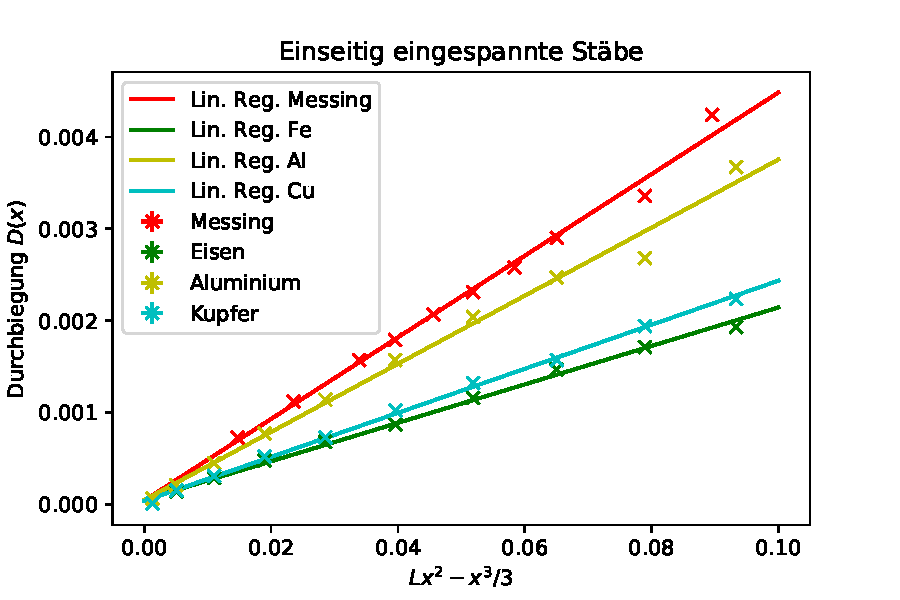
\includegraphics{einseitig.pdf}
    \caption{Absenkung eines einseitig eingespannten Stabes.}
    \label{fig:einseitigu}
  \end{figure}
\begin{table}
    \centering
      \caption{In der Tabelle sind die Parameter der Ausgleichsgraden dargestellt.}
      \label{tab:parameter1}
      \sisetup{table-format=1.2}
      \begin{tabular}{S[table-format=3.2] S S S S S S S S [table-format=3.2]}
        \toprule
        {Nr.} & {Material}&{$a$ /m^2}&{$b$ /m}\\
        \midrule
        1 & {Messing}   &{$$(0.0444 \pm 0.0015)$$}&{$$(0.0000 \pm 0.0001)$$}\\
        2 & {Eisen}     &{$$(0.0209 \pm 0.0005)$$}&{$$(0.0001 \pm 0.0000)$$}\\
        3 & {Aluminium} &{$$(0.0371 \pm 0.0013)$$}&{$$(0.0000 \pm 0.0001)$$}\\
        4 & {Kupfer}    &{$$(0.0240 \pm 0.0004)$$}&{$$(0.0000 \pm 0.0000)$$}\\
        \bottomrule
      \end{tabular}
    \end{table}
Die Elastizitätsmodule ergeben sich durch Vergleich der funktion der Ausgleichsgraden mit 
\autoref{eq:eins} zu:
\begin{center}
    \begin{equation}
      \label{eq:elastizitaet}  
      E=\frac{mg}{2Ia}
    \end{equation}
\end{center}
mit der Steigung $a$ der Ausgleichsgraden aus \autoref{tab:parameter1}. Es ergeben sich also
folgende Elastizitätsmodule:
\begin{center}
    $E_{Mes}=(102.0\pm 4.0)\si[]{GPa}$\\
    $E_{Fe}=(216.0\pm 7.0)\si[]{GPa}$\\
    $E_{Al}=(71.0\pm 2.9)\si[]{GPa}$\\
    $E_{Cu}=(111.2\pm 2.8)\si[]{GPa}$\\
\end{center}
\subsection{Beidseitig eingespannter Stab}
Das Elastizitätsmodul kann auch berechnet werden wenn der Stab beidseitig eingepannt wird und die 
Masse in der Mitte bei $L/2=\SI[]{0.275}[]{m}$ angehängt wird. Im Folgenden wird die linke Seite des Stabes aufgelegt und
die rechte Seite eingespannt. Die Absenkungen der linken Seite werden in \autoref{fig:beidseitig11} gegen den Term
$3L^2x-4x^3$ und die rechte Seite in \autoref{fig:beidseitig22} gegen den Term $4x^3-12Lx^2+9L^2-L^3$ aufgetragen.
Analog zu \autoref{sec:nr1} werden Ausgleichsgraden durch die Punkte gelegt die zugehörigen Parameter sind in
\autoref{tab:parameter2} dargestellt.
\begin{figure}
    \centering
    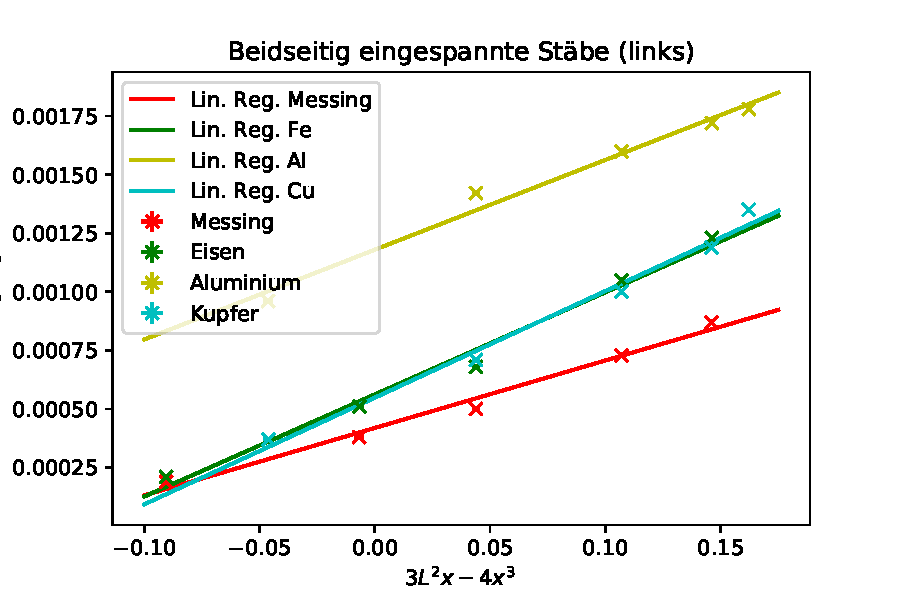
\includegraphics{beidseitig1.pdf}
    \caption{Absenkung der linken Seite eines beidseitig eingespannten Stabes.}
    \label{fig:beidseitig11}
  \end{figure}
  \begin{figure}
    \centering
    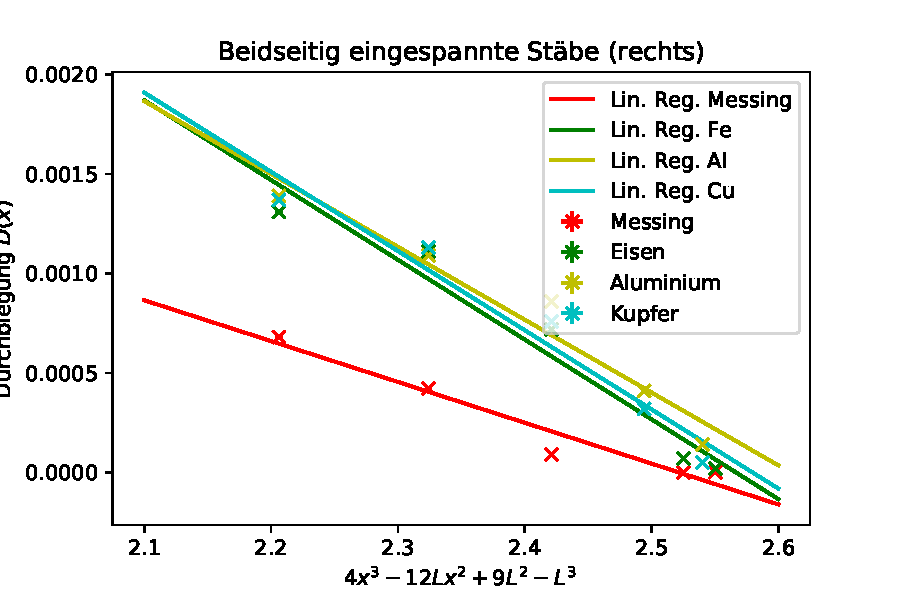
\includegraphics{beidseitig2.pdf}
    \caption{Absenkung der rechten Seite eines beidseitig eingespannten Stabes.}
    \label{fig:beidseitig22}
  \end{figure}

  \begin{table}
    \centering
      \caption{In der Tabelle sind die Parameter der Ausgleichsgraden dargestellt.}
      \label{tab:parameter2}
      \sisetup{table-format=1.2}
      \begin{tabular}{S[table-format=3.2] S S S S S S S S [table-format=3.2]}
        \toprule
        {Nr.} & {Material}&{$a_{links}$ /m^2}&{$b_{links}$ /m}&{$a_{rechts}$ /m^2}&{$b_{rechts}$ /m}\\
        \midrule
        1 & {Messing}   &{$$(0.0029 \pm 0.0002)$$}&{$$(0.0004 \pm 0.0000)$$}&{$$(0.0020 \pm 0.0002)$$}&{$$(0.0051 \pm 0.0006)$$}\\
        2 & {Eisen}     &{$$(0.0044 \pm 0.0003)$$}&{$$(0.0006 \pm 0.0000)$$}&{$$(0.0040 \pm 0.0005)$$}&{$$(0.0102 \pm 0.0012)$$}\\
        3 & {Aluminium} &{$$(0.0038 \pm 0.0003)$$}&{$$(0.0012 \pm 0.0000)$$}&{$$(0.0036 \pm 0.0004)$$}&{$$(0.0095 \pm 0.0011)$$}\\
        4 & {Kupfer}    &{$$(0.0046 \pm 0.0003)$$}&{$$(0.0005 \pm 0.0000)$$}&{$$(0.0039 \pm 0.0005)$$}&{$$(0.0102 \pm 0.0012)$$}\\
        \bottomrule
      \end{tabular}
    \end{table}

    Nun kann ein Vergleich analog zu \autoref{sec:nr1} angestellt werden welcher zur Formel zur
    berechnung des Elastizitätsmoduls führt. Sie lautet:
    \begin{center}
        $E=\frac{mg}{48Ia}$
    \end{center}
    Dabei wird für Messing eine Masse von $m=(2.859\pm 0.0001)\si[]{kg}$ und für die anderen drei Materialien
    eine Masse von $m=(4.298\pm 0.0001)\si[]{kg}$ angehängt. Das führt zu den in \autoref{tab:ergebnisse} dargestellten
    Ergebnissen. Der jeweils zugehörige Fehler berechnet sich über \autoref{eq:gaussfehler}.

    \begin{table}
        \centering
          \caption{In der Tabelle sind die berechneten Elastizitätsmodule eines beidseitig aufliegenden Stabes aufgeführt.}
          \label{tab:ergebnisse}
          \sisetup{table-format=1.2}
          \begin{tabular}{S[table-format=3.2] S S S S S S S S [table-format=3.2]}
            \toprule
            {Nr} & {Material}&{$E_{links}$ /GPa}&{$E_{rechts}$ /GPa}\\
            \midrule
            1 & {Messing}   &{$$(413\pm 30)$$}&{$$(580\pm 80)$$}\\
            2 & {Eisen}     &{$$(411\pm 29)$$}&{$$(450\pm 60)$$}\\
            3 & {Aluminium} &{$$(275\pm 22)$$}&{$$(290\pm 40)$$}\\
            4 & {Kupfer}    &{$$(231\pm 16)$$}&{$$(265\pm 34)$$}\\
            \bottomrule
          \end{tabular}
        \end{table}

\subsection{Vergleich der Elastizitätsmodule}
\label{sec:vergleich}
In \autoref{tab:ergebnisse2} sind die auf beide Arten berechneten Elastizitätsmodule 
dargestellt. Sie weichen untereinander stark ab. Mögliche Gründe dafür sind in
\autoref{sec:diskussion} zu finden.
\begin{table}
    \centering
      \caption{In der Tabelle sind alle berechneten Elastizitätsmodule dargestellt.}
      \label{tab:ergebnisse2}
      \sisetup{table-format=1.2}
      \begin{tabular}{S[table-format=3.2] S S S S [table-format=3.2]}
        \toprule
        {Nr} & {Material} & {$E_{einseitig}$ /GPa} & {$E_{links}$ /GPa} & {$E_{rechts}$ /GPa}\\
        \midrule
        1 & {Messing}   &{$$(102.0\pm 4.0)$$}&{$$(413\pm 30)$$}&{$$(580\pm 80)$$}\\
        2 & {Eisen}     &{$$(216.0\pm 7.0)$$}&{$$(411\pm 29)$$}&{$$(450\pm 60)$$}\\
        3 & {Aluminium} &{$$(71.0 \pm 2.9)$$}&{$$(275\pm 22)$$}&{$$(290\pm 40)$$}\\
        4 & {Kupfer}    &{$$(111.2\pm 2.8)$$}&{$$(231\pm 16)$$}&{$$(265\pm 34)$$}\\
        \bottomrule
      \end{tabular}
    \end{table}

    